%%
%% This is file `mcmthesis-demo.tex',
%% generated with the docstrip utility.
%%
%% The original source files were:
%%
%% mcmthesis.dtx  (with options: `demo')
%% 
%% -----------------------------------
%% 
%% This is a generated file.
%% 
%% Copyright (C)
%%     2010 -- 2015 by Zhaoli Wang
%%     2014 -- 2016 by Liam Huang
%% 
%% This work may be distributed and/or modified under the
%% conditions of the LaTeX Project Public License, either version 1.3
%% of this license or (at your option) any later version.
%% The latest version of this license is in
%%   http://www.latex-project.org/lppl.txt
%% and version 1.3 or later is part of all distributions of LaTeX
%% version 2005/12/01 or later.
%% 
%% This work has the LPPL maintenance status `maintained'.
%% 
%% The Current Maintainer of this work is Liam Huang.
%% 
\documentclass{mcmthesis}
\mcmsetup{CTeX = false,   % 使用 CTeX 套装时,设置为 true
        tcn = 34317, problem = A,
        sheet = true, titleinsheet = true, keywordsinsheet = true,
        titlepage = true, abstract = true}
\usepackage{palatino}
\usepackage{booktabs}
\usepackage{amsmath}
\title{Stochastic and Dterministic Models of the Eradication of
Ebola in West Africa}
\date{\today}
\begin{document}
\begin{abstract}
As a number fo Global Village, we do out bset to help \textbf{eradicate} Ebola

First, we develop a stage-structrured model of Ebola Propagation. In the model, we
consider the susceptible, the exposed, the infected whose disease is not advanced, the infected whose
disease is serious, the removed and the dead. The model is good at predicting near future cases` number
but fails in predicting far future cases` number. Then we take hospital into consideration and add 7 more
parameters, then we do simulation once again. Finally, we get a better result that the model well predicts
the future cases. For example, the model predicts there are 4000 total cases and 2500 death cases in Guinea,
9509 total cases and 4166 death case in Liberia, 12556 total cases and 2922 death cases in Sierra Leone up to 
April, $1^{st}$, 2015.

Second, we determine the location fo delivery. We invoke clustering method to divide the most serious region, namely,
West Africa into three parts, Guinea, Liberia and Sierra Leone, According to locations of provincial capital, we use clustering
method once again to divide a country into several clusters. Then we adopt P-Center Method to determine a location of 
delivery in each cluster. We find there are two kinds of ways to choose. One is one-way route and the other is circular route. As for
one-way route, in some ways, is a little bit similar to TSP problem, we use mix integer programming to find an optimal circular route by
Lingo Software and each location of delivery has two optimal circular routes. The result is that there are 3 locations of delivery in Guinea,
1 location of delivery in Liberia and i lcoation of delivery in Sierra Leone.

Third, we know from the stages-structrured model the Ebola cannot stop spreading by itself, Since we are going to eradicate Ebola, we
must use medicine and vaccine to stop Ebola. Medicine mainly influences the number of the susceptible while vaccine mainly influences
the number of the infected whose disears is not advanced, in this way, we can eradicate Ebola. As for speed of manufacturing, we consider there is
a linear equation between the speed and time because the amount of medicine is too rare to meet the requrement of patients. And this situation continues
until the requirement is met. We can calculate the speed  by the parameter in the linear equation. And we allocate medicine to different places by ratio of
the infected number in that place to the number in three West African countries. Thus, we successfully stop Ebola from sperading.
\begin{keywords}
SEIIRF Model TSP Model Clustering Method Ebola Evaluating
\end{keywords}
\end{abstract}
\maketitle
\tableofcontents
\newpage

\section{Introduction}
Ebola, a familiar but strange word to us. When the Ebola virus out broke in West Africa and caused plenty of deaths, no one
would imagine the disastrous scene without mercy. And, of course, no one believe that word 'Ebola' just originated from a peaceful and 
beautiful river -- Ebola River in Congo. Contrary to its attracting meaning, it is true that the Ebola virus do take lots of victims`
live away. Countries all over the world, thus, have taken strategies, more specifically, distribute health works to disease-torn countries, speed up
the development of medicine and establish feasible delivery systems to contain Ebola propagation. 
\subsection{Aims are changing now}
The battle against Ebola will cost us heavily for sure, but human being are not
easily defeated. Although Ebola virus is fatal, we have methods. The WMA (World Medical Association) has announced that
 they have developed medicine to cure Ebola, but at another it is the result of human nature. We know calling the command
center to take away the sick is equally hard. It is out \cite{5}
\subsection{Our understanding of the words}
The battle against Ebola will cost us heavily for sure, but human beings are not easily defeated. Although Ebola virus is
fatal.

\textbf{Spread of the Disease:}We consider this sub-problem as a requirement to analyze Ebola propagation process and predict
future cases, includeing total cases and death cases in th e three West African countreies, such as in the United States or in The
United Kingdom, good health condition and developed facilities can contain the cases well, so in this paper, we mainly discuss Ebola
cases in West African. 
\begin{itemize}
\item minimizes the discomfort to the hands, or
\item maximizes the outgoing velocity of the ball.
\end{itemize}
We focus exclusively on the second definition.

\begin{center}
\begin{tabular}{ccccc}
  \toprule
  number & sex & old & tall/cm & weight/kg \\
  \midrule
  1 & F & 14 & 156 & 42 \\
  2 & F & 16 & 158 & 45 \\
  3 & M & 14 & 162 & 48 \\
  4 & M & 18 & 170 & 50 \\
  \bottomrule
\end{tabular}
\end{center}

\begin{itemize}
\item the initial velocity and rotation of the ball,
\item the initial velocity and rotation of the bat,
\item the relative position and orientation of the bat and ball, and
\item the force over time that the hitter hands applies on the handle.
\end{itemize}
\begin{itemize}
\item the angular velocity of the bat,
\item the velocity of the ball, and
\item the position of impact along the bat.
\end{itemize}
\emph{center of percussion} [Brody 1986]

\begin{Theorem} \label{thm:latex}
\LaTeX
\end{Theorem}
\begin{Lemma} \label{thm:tex}
\TeX .
\end{Lemma}
\begin{proof}
The proof of theorem.
\end{proof}

\subsection{Other Assumptions}
\begin{itemize}
\item
\item
\item
\end{itemize}

%%表格
\begin{center}
\begin{tabular}{| > {$}r < {$}|>{\setlength \parindent{2em}}m{15em}|
  > {\centering \arraybackslash}m{4em}|}
\hline
\pi & ok sij ajkjs ak j & normal \\
\hline
\aleph
\aleph & lijkjk & normal \\
\hline
\end{tabular}
\end{center}

\begin{equation}
  a + b = b + a \label{eq:commutative}
\end {equation}


\section{Analysis of the Problem}
\begin{figure}[h]
\small
\centering
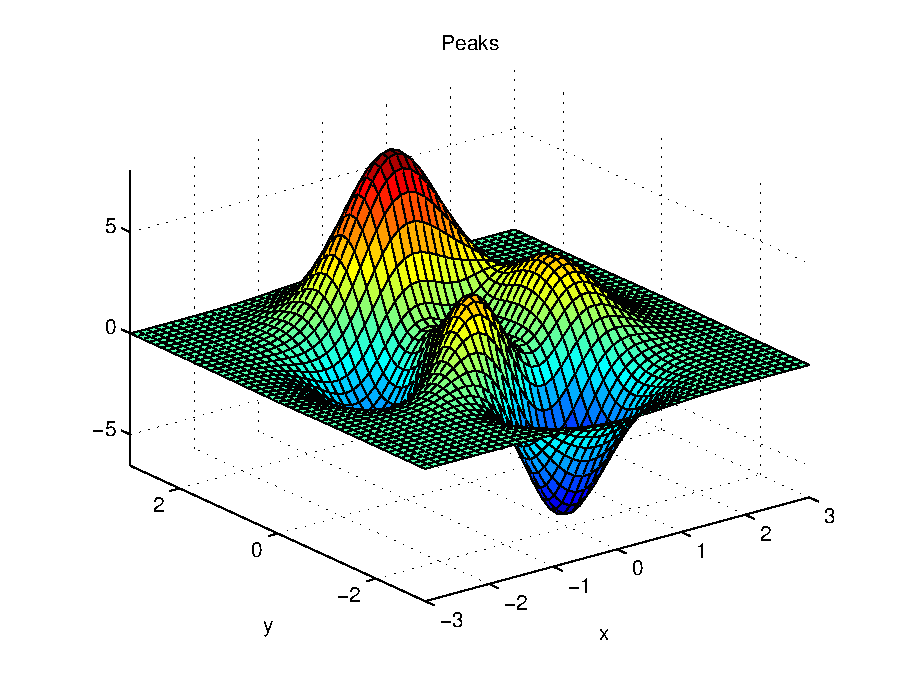
\includegraphics[width=12cm]{mcmthesis-aaa.eps}
\caption{aa} \label{fig:aa}
\end{figure}

\eqref{aa}
\begin{equation}
a^2 \label{aa}
\end{equation}

\[
  \begin{pmatrix}{*{20}c}
  {a_{11} } & {a_{12} } & {a_{13} }  \\
  {a_{21} } & {a_{22} } & {a_{23} }  \\
  {a_{31} } & {a_{32} } & {a_{33} }  \\
  \end{pmatrix}
  = \frac{{Opposite}}{{Hypotenuse}}\cos ^{ - 1} \theta \arcsin \theta
\]

\[
  p_{j}=\begin{cases} 0,&\text{if $j$ is odd}\\
  r!\,(-1)^{j/2},&\text{if $j$ is even}
  \end{cases}
\]

\[
  \arcsin \theta  =
  \mathop{{\int\!\!\!\!\!\int\!\!\!\!\!\int}\mkern-31.2mu
  \bigodot}\limits_\varphi
  {\mathop {\lim }\limits_{x \to \infty } \frac{{n!}}{{r!\left( {n - r}
  \right)!}}} \eqno (1)
\]

\section{Calculating and Simplifying the Model  }

\section{The Model Results}

\section{Validating the Model}

\section{Conclusions}

\section{A Summary}

\section{Evaluate of the Mode}

\section{Strengths and weaknesses}
\[
\mathcal{F}(x) = \sum_{k = 0}^\infty
\oint_0^1 f_k(x,t) \, \mathrm{d}t
\]

\subsection{Strengths}
\begin{itemize}
\item \textbf{Applies widely}\\
This  system can be used for many types of airplanes, and it also
solves the interference during  the procedure of the boarding
airplane,as described above we can get to the  optimization
boarding time.We also know that all the service is automate.

\item \textbf{Improve the quality of the airport service}\\
Balancing the cost of the cost and the benefit, it will bring in
more convenient  for airport and passengers.It also saves many
human resources for the airline. 

\item \textbf{equation}

\[
A_ij = 2^{i+j}
\]
$A_i^k = B_i^k$

\item $max f(n) = \sum_{i = 0}^n A_i$ ok the last equation is $\int_0^1 f(t) \dif t
 = \iint_D g(x,y) \dif x \dif y$
\end{itemize}


\subsection{test2}
\[
 \iiint\limits_D \mathrm{d}f 
  = \max\nolimits_D g
\] $\sum\limits_{i = 0}^n A_i$ is not better than $\sum_{x = 0}^n A_i$
$\overline{a+b} = \overline a + \overline b$ $\underline a = (a_0, a_1, a_2, \dots)$

$ \overline{\underline{\underline a}
+ \overline{b}^2} - c^{\underline n}$

$\rlap{$\overbrace{\phantom{a \to b}}$} a \to \underbrace{b \to c}$\\
$a+\rlap{$\overbrace{d+\phantom{c+d}}^m$}\underbrace{c+d+e}_n+f$

\begin{thebibliography}{99}
\bibitem{1} D.~E. KNUTH   The \TeX{}book  the American
Mathematical Society and Addison-Wesley
Publishing Company , 1984-1986.
\bibitem{2}Lamport, Leslie,  \LaTeX{}: `` A Document Preparation System '',
Addison-Wesley Publishing Company, 1986.
\bibitem{3}\url{http://www.latexstudio.net/}
\bibitem{4}\url{http://www.chinatex.org/}
\bibitem{5}ok
\end{thebibliography}


\section{test1}


\section{test2}


\section{appendix}



\begin{appendices}

\section{First appendix}


Here are simulation programmes we used in our model as follow.\\

\textbf{\textcolor[rgb]{0.98,0.00,0.00}{Input matlab source:}}
\lstinputlisting[language=Matlab]{./code/mcmthesis-matlab1.m}

\section{Second appendix}

some more text \textcolor[rgb]{0.98,0.00,0.00}{\textbf{Input C++ source:}}
\lstinputlisting[language=C++]{./code/ex10.cpp}

\end{appendices}
\end{document}

%% 
%% This work consists of these files mcmthesis.dtx,
%%                                   figures/ and
%%                                   code/,
%% and the derived files             mcmthesis.cls,
%%                                   mcmthesis-demo.tex,
%%                                   README,
%%                                   LICENSE,
%%                                   mcmthesis.pdf and
%%                                   mcmthesis-demo.pdf.
%%
%% End of file `mcmthesis-demo.tex'.
